% Trailing asterisk to suppress section number
\section*{Task 1: SQL injections}

\subsection*{Exercises:}
\begin{enumerate}
\item \exercise{Perform SQL injections in at least one input field on the BadStore website. In the lab report, give the injections
and the output/result. Explain how each injection works word for word, and why it works.}

We chose to perform SQL injections in the input box for the email address on the login page, shown in the upper half of \autoref{fig:sql1}. The result---being logged on as the administrator---is shown in the lower half of the figure.
\begin{figure}[h!]
	\caption{SQL Injection and Logged in as Administrator}
        \label{fig:sql1}
	\centering 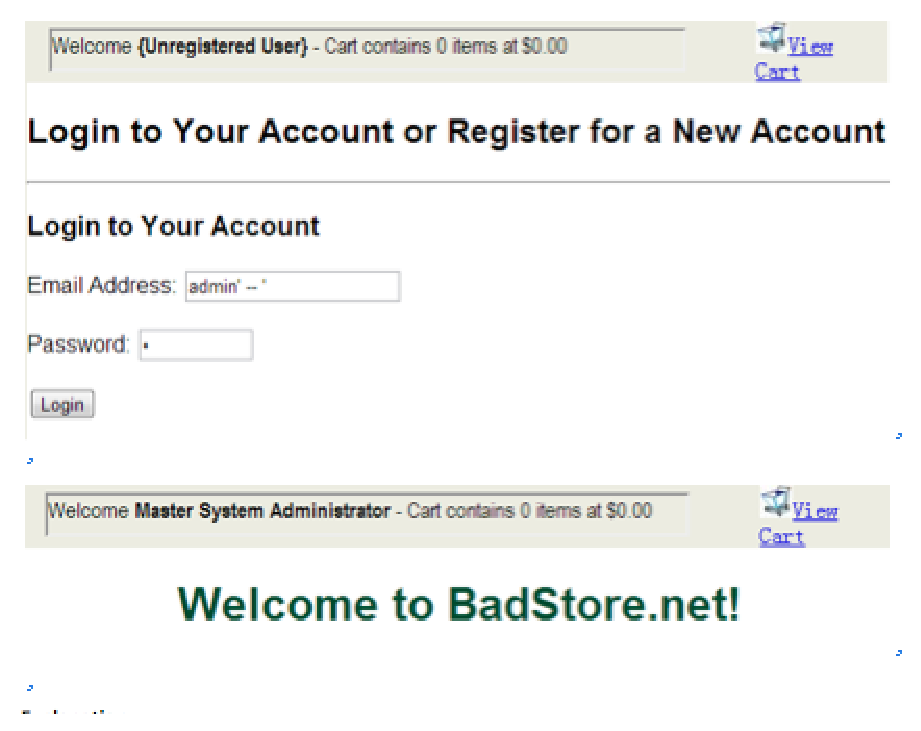
\includegraphics[height=2.5in]{sqli1}
\end{figure}
  
  \textbf{Explanation} Without injection, the SQL code executed when a login request is made is believed to be \lstinline{SELECT * FROM user WHERE EmailAddress = 'emailaddress' AND Password = 'password'}. Then during the injection, we input \lstinline{admin' -- '} in the text box for the email address and some arbitrary password in the text box for the password. The WHERE condition is altered into \lstinline{WHERE EmailAddress = 'admin' -- '' AND Password = 'password'}, where the part following the two dashes is interpreted as a SQL comment. In other words, the WHERE condition is turned into \lstinline{WHERE EmailAddress = 'admin'}. Thus there is no need for a password and we can directly log into the admin account.

One would think that the apostrophe following the two dashes would be ignored and thus not be necessary to include, but without it, an error message is received. Running \program{nmap} on the BadStore server shows that it is running MySQL 4.1.7. There appears to have been several bugs in MySQL related to apostrophes in comments\cite{quoteComment1}\cite{quoteComment2}, and we believe that a similar bug may be the cause of the odd behavior experienced on BadStore.
\item \exercise{Make sure that you are logged on to the pen test lab via VPN. Perform SQL injection on 192.168.2.134 in the
pen test lab. What happens? In the lab report, explain how the SQL injection works and its result.}

The login page for host \ip{192.168.2.134} and that it was was circumvented successfully using SQL injection is shown in \autoref{fig:sql2}.
\begin{figure}[h!]
	\caption{SQL Injection and the Result}
        \label{fig:sql2}
	\centering 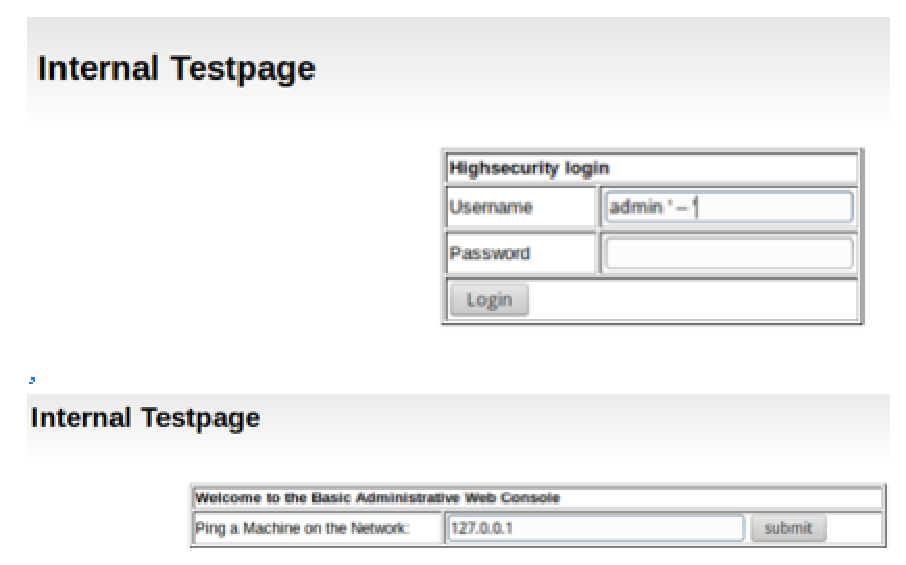
\includegraphics[height=2.5in]{sqli2}
\end{figure}
\\
  \textbf{Explanation} The underlying SQL code for the login screen for host \ip{192.168.2.134} is believed to be the same as before: without injection, the SQL code is thought to be \lstinline{SELECT * FROM user WHERE UserName = 'username' AND Password = 'password'}. Then during the injection, we input \lstinline{admin '-- '} in the text box for the username and some arbitrary password in the text box for the password. The WHERE condition is altered into \lstinline{WHERE UserName = 'admin' -- ' AND Password = 'password'} (or equivalently, \lstinline{WHERE UserName = 'admin'}). So there is no need for a password and we can directly log into the admin account.

After having successfully performed the SQL injection, we were presented an internal test page, which is shown in the lower half of \autoref{fig:sql2}. On the test page, we can ping machines on the network by entering an IP address in the text box and clicking the submit button.
\item \exercise{What could a system administrator do to prevent SQL injections such as the ones you just did? Explain carefully
in the lab report.}

The system administrator can use so-called \textit{prepared statements} to prevent SQL injections. A prepared statement, which is also called a parametrized statement, is a SQL query with variables inside of it\cite{preparedStatement}. That is to say, we prepare the query with blank spots to fill and it will automatically protect the query from SQL injection. An example of how to use a prepared statement in PHP is shown below\cite{php}:
  \begin{lstlisting}[language = php]
    stmt = dbh->prepare("INSERT INTO REGISTRY (name, value) VALUES (:name, :value)");
    stmt->bindParam(':name', name);
    stmt->bindParam(':value', value);
  \end{lstlisting}

  In the previous exercises, a username and a password have been supplied by the user. That is, the queries have been of the form
\begin{lstlisting}
  SELECT * FROM user WHERE UserName = 'admin' AND Password = 'test'
\end{lstlisting}

A prepared statement for the query above could be arranged as follows:
  \begin{lstlisting}
    prepare("SELECT * FROM user WHERE UserName = :username AND Password = :password");
    bind(':username', username);
    bind(':password', password);
  \end{lstlisting}
  
  There are two variables in the prepared statement: username and password. Without injection, for instance with the username \lstinline{admin} and the password \lstinline{test}, the SQL query for logging on would be \lstinline{SELECT * FROM user WHERE username = 'admin' AND password = 'test'}. During an injection attempt, for instance with the username \lstinline{admin' -- '} and password \lstinline{123}, the SQL query becomes \lstinline{SELECT * FROM user WHERE username = 'admin\' -- ' AND password = '123'}. That is, the username is interpreted as the very username that was entered: \verb|admin' -- |. This is because the binding system will automatically change the input to protect the query. Seeing as there is no user by the name \verb|admin' -- |, the login fails, and the attempt at SQL injection is unsuccessful. 
\item \exercise{Explain the below joke in your lab report in a boring, technical and thorough way, clarifying what happened
to the school and what they should do about it.}

The school lost all the student records because the table Students in the database is dropped by SQL injection. The SQL statement intended to be executed can be assumed to be of the form \lstinline{INSERT INTO Students VALUES ('Robert');}. The SQL injection had this query altered into the following two statements and comment: \lstinline{INSERT INTO Students VALUES ('Robert'); DROP TABLE Students; --');}. When the query is executed, the table Students will be dropped.

  What the school should do is to sanitize the database inputs by utilizing prepared statements as mentioned above. They can create the prepared statement as follows:
  \begin{lstlisting}
    prepare("INSERT INTO Students VALUES (':name')");
    bind(':name',name);
  \end{lstlisting}

\end{enumerate}
